%%%%%%%%%%%%%%%%%%%%%%%%%%%%%%%%%%%%%%%%%%%%%%%%%%%%%%%%%%%%
% Document settings
\documentclass{ACGSeminar}

%%%%%%%%%%%%%%%%%%%%%%%%%%%%%%%%%%%%%%%%%%%%%%%%%%%%%%%%%%%%
% Own Packages

%%%%%%%%%%%%%%%%%%%%%%%%%%%%%%%%%%%%%%%%%%%%%%%%%%%%%%%%%%%%
% Own Definitions
\newcommand{\comment}[1]{}


%%%%%%%%%%%%%%%%%%%%%%%%%%%%%%%%%%%%%%%%%%%%%%%%%%%%%%%%%%%%
% BibTex
\bibliography{references}

%%%%%%%%%%%%%%%%%%%%%%%%%%%%%
% Hyphenations here
%%%%%%%%%%%%%%%%%%%%%%%%%%%%%
\hyphenation{Sa-tan-arch-aeo-li-deal-co-hell-ish}

%%%%%%%%%%%%%%%%%%%%%%%%%%%%%
% Title, Author, etc.

\begin{document}

\title{Re: Deep G-Buffers for Stable Global Illumination Approximation}

\author{Ferit Tohidi Far}

\maketitle

%%%%%%%%%%%%%%%%%%%%%%%%%%%%%%%%%%%%%%%%%%%%%%%%%%%%%%%%%%%%
% Abstract

\begin{abstract}%
G-buffers can be used to efficiently render images with large amounts of light sources. This is possible thanks to a process called "deferred rendering". Using 
only g-buffers, we are only able to compute local illumination, which forces us to find a way to achieve sought after visual and lighting effects like global 
illumination. By using deep g-buffers we can approximate global illumination in a way that is more efficient than traditional methods like pathtracing, 
while of course not being physically accurate. We can make up for it, though, by also approximating visual effects like ambient occlusion, color bleeding, reflections, 
depth of field and motion blur to create an acceptable interactive realtime result, which is - as of now - simply impossible with physically accurate methods on 
average hardware.
\end{abstract}

\keywords{nvidia, g-buffer, deep g-buffer, pathtracing, global illumination approximation, deferred shading, deferred rendering}
\tableofcontents

\label{cha:references}

\newpage

%%%%%%%%%%%%%%%%%%%%%%%%%%%%%%%%%%%%%%%%%%%%%%%%%%%%%%%%%%%%
% Introduction
\label{cha:introduction}
\section{Global illumination}
	Global illumination is a lighting effect that is achieved by not only computing direct light, but also indirect light, meaning that it is neccesary to take
	into account how light reflects and carries information (in the most basic case: color).
	\subsection{Physically correct methods}
	In order to generate physically correct lighting, which is a requirement for creating photorealistic images, we need to solve the rendering equation
	$$ L_o(\omega) = L_e(\omega) + \int_\Omega f(\omega, \omega')L_i(\omega')cos(n, \omega') \partial \omega' $$
	where 
	\begin{center}
		\begin{align*}
			&L_o(\omega) \text{ is the outgoing light in direction } \omega\text{,}\\
			&L_e(\omega) \text{ is the emmited light in direction } \omega\text{,}\\
			&f(\omega, \omega') \text{ is the BRDF\footnotemark} \text{,}\\
			&L_i(\omega') \text{ is the incoming light from direction } \omega'\\
			&\text{and } cos(n, \omega') \text{ is lambert reflectance\footnotemark}  \text{ .}
		\end{align*}
	\end{center}
	\addtocounter{footnote}{-1}
	\footnotetext{The bidirectional random distribution function basically describes the reflection/refraction of a ray on surface.}%
	\stepcounter{footnote}
	\footnotetext{Lambert reflectance describes the attentuation of light on diffuse objects based on the lights incident angle.}%
	The most popular method for achieving this is pathtracing \cite{P2PATH}.
	\subsubsection{Pathtracing}
		Pathtracing solves the rendering equation by first sending camera rays through each individual pixel of the image plane and then tracing the ray back to the light source. If the lamp is hit the pixel gets painted painted with color, else black. Direct consequences of this are soft shadows and ambient occlusion. A maximum hop number caps the amount of times a ray is able to reflect. A hop number larger than 1 (3 in most simple cases is sufficient, but it is dependent on the complexity of the scene) allows for global illumination. The reflections and refractions are essentially determined by the BRDF, which not only means that objects can be transparent, but we also get caustics\footnote{Caustics are areas with concentrated light. This happens due to light refracting.}. With each surface a ray hits it carries information from that surface, e.g. its color, and reflects it onto the next surface it hits. This causes color bleeding. What all these visual effects describe is explained in section 4.
	\subsection{Computational difficulties of physically correct methods}
	Since we have to take into account thousands of samples of every ray of light with its reflections, the computational difficulty becomes apparent \cite{DST}. Because of this, it is nearly impossible to achieve real time rendering using physically correct methods on an average system. This forces game engines to stick to approximating global illumination and visual effects since it is way more efficient to compute. Add multiple light sources to the scene, and the computational requirements are going to blow up. Deferred rendering, specifically deferred shading, counters this problem at the cost of having to compute transparency using depth peeling.
	% TODO insert time-complexity of pathtracing and time-complexity of deferred-rendering for comparison

\section{Deferred rendering}
	Graphics pipelines describe each step that has to be done in order to render an image. Within a pipeline it is possible in some cases to defer steps to a later stage. It is conventional to use GPU's for applications that rely heavily on rendering images. There is no universal graphics pipeline, because these are dependent on the GPU that is used, which means it is convenient that there exist API's like OpenGL that try to generalize the steps that need to be taken in order to render an image and map them to compatible GPU's. This means that most GPU dependent applications abide by the graphics pipeline as described by, for instance, OpenGL (figure \ref{fig:graphics_pipeline}).
	\begin{figure}[htb!]%
	\begin{center}%
		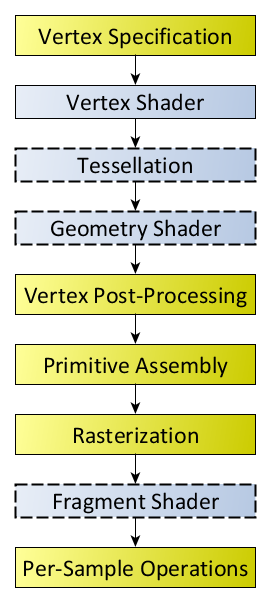
\includegraphics[height=7cm]{img/graphics_pipeline.png}
	\end{center}%
	\caption{The OpenGL graphics pipeline.}%
	\label{fig:graphics_pipeline}%
	\end{figure}%
	\subsection{How deferred shading handles lighting more efficiently}
		%TODO insert example of how a graphics pipeline could look, possible an image
		The goal of deferred shading is to defer the shading stage. %TODO insert information about graphics pipeline
		Instead of shading right away, we compute necessary geometry buffers (g-buffers) in a first pass that we call "geometry pass" and cache 
		them for later use in the second pass which we call "shading (or lighting) pass". With forward shading we would have to compute the shading for every fragment of every object for all light-sources in a single pass. The shading is applied regardless wether the fragment is visible at the end or not. This means that the time complexity of computing the shading is $O(amount_{polygons} \cdot amount_{fragments} \cdot amount_{lights})$. If we apply deffered shading, however, we do not force ourselves to shade every fragment as soon as it has been computed, instead we wait until we find the closest fragment so to say. Finding the closest fragment is called "solving the visibility problem". This is solved during the geometry pass when filling the z-buffer with its respective z-values, which can be computed by performing perspective correct interpolation between the vertices of the current polygon (in most cases triangles). The z-buffer, along with all other buffers that are collected, are continuously updated if a closer fragment for the same pixel is found, which solves the visibility problem. Now all the fragments that we shade are only going to be shaded once, which means for the time complexity that the shading is done in $O(amount_{fragments} \cdot amount_{lights})$, allowing us to render more light-sources at the expense of passing around g-buffers. For all practical purposes, g-buffers have to at least consist of a frame-buffer, a normal-buffer and a z-buffer. Using only these g-buffers, it is possible to render an image with basic shading.

\section{Geometry-buffer (g-buffer)}
	Each geometry-buffer stores information of some sort for each individual pixel, meaning that they are all two-dimensional arrays.
	\subsection{Frame-buffer}%
		Color-values of fragments are stored in the frame-buffer. It basically stores the rendered image without fragment-shading\footnote{Fragment-shading is ...} applied to it.% 
		\begin{figure}[htb!]%
			\begin{center}%
				
\includegraphics[width=7cm]{img/frame_buffer.png}
			\end{center}%
			\caption{Example of a frame-buffer (also called image-buffer). It shows a cornell box with white walls containing two blue cuboids.}%
			\label{fig:frame_buffer}%
		\end{figure}%
	\subsection{Z-buffer}
		The z-buffer stores depth values of fragments. These are needed to determine which surfaces are closest and visible to the camera. If two different fragments\footnote{A fragment is a point on a surface in 3d space (worldspace\footnotemark)} have the same x and y coordinates in screenspace\footnotemark, then the fragment with the smaller z-value is supposed to be in front of the other. This buffer is also used for screenspace visual effects like screen space ambient occlusion. 
		\addtocounter{footnote}{-1}
		\footnotetext{Worldspace is ...}
		\stepcounter{footnote}
		\footnotetext{Screenspace is ...}
		\begin{figure}[htb!]%
			\begin{center}%
				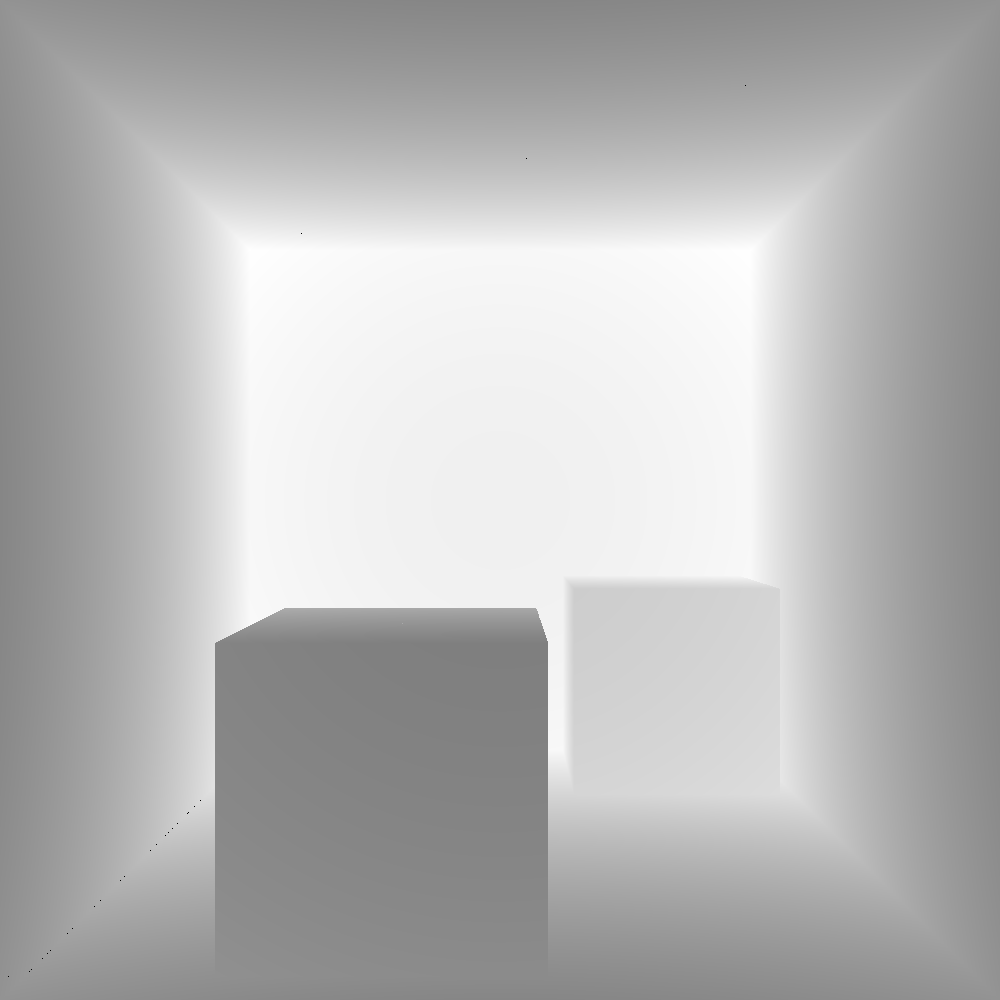
\includegraphics[width=7cm]{img/z_buffer.png}
			\end{center}%
			\caption{Example of a z-buffer. Since the z-buffer only stores distances as float values instead of actual colors they are interpreted as the grayscale value deduced by dividing each
			distance by the maximum distance from the cameras point of view.}%
			\label{fig:z_buffer}%
		\end{figure}%
	\subsection{Normal-buffer}
		The normal-buffer stores surface-normals that are mostly used to determine reflection and refraction directions. They are also used for light attentuation, since they determine the cosine of the surface and the incident light and a larger cosine means lighter light and vice versa (lambert reflectance).
		\begin{figure}[htb!]%
			\begin{center}%
				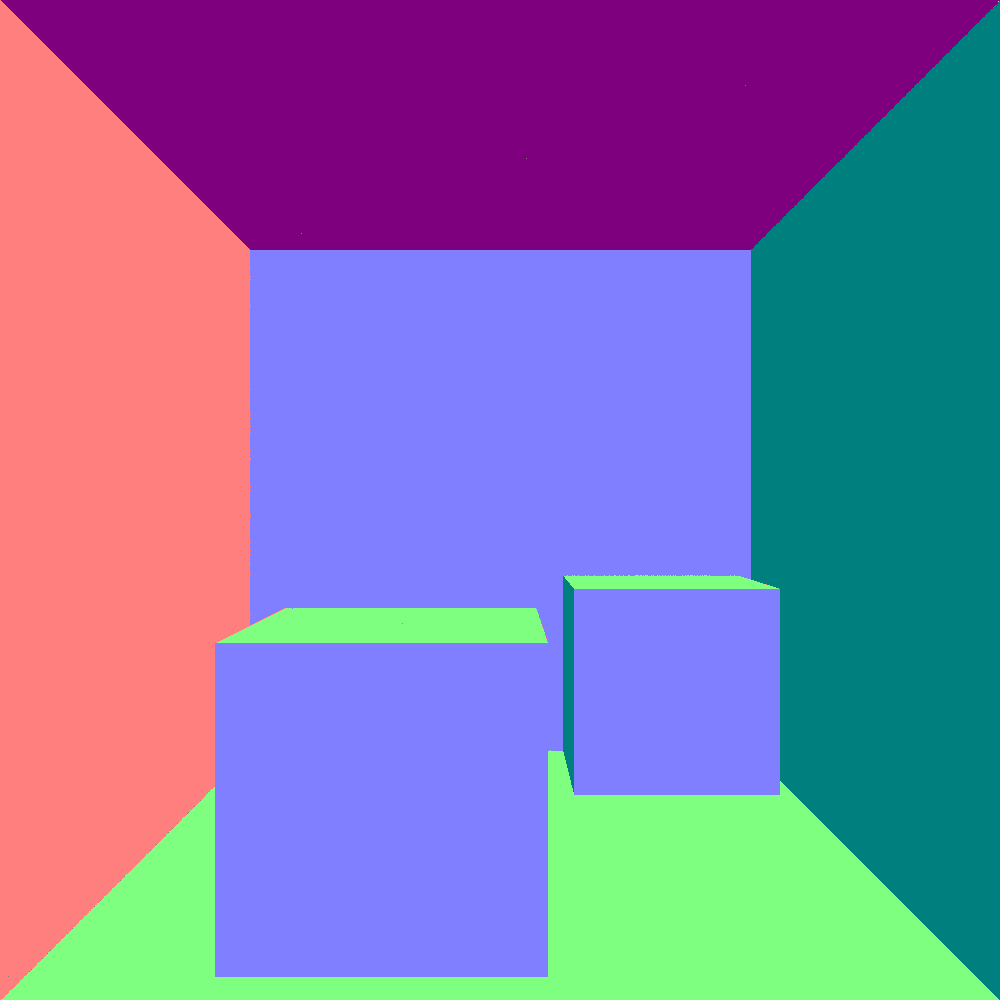
\includegraphics[width=7cm]{img/normal_buffer.png}
			\end{center}%
			\caption{Example of a normal-buffer. Normal vectors are usually normalized, meaning their values range from 0 to 1. Multiplying them with 255 gives us an RGB color. Since negative normals
			would cause negative RGB values we just take the absolute values.}%
			\label{fig:normal_buffer}%
		\end{figure}%
		Note that there are more possible buffers to choose from, but the three that were mentioned are the most essential in every g-buffer.
	\subsection{Computing local illumination using g-buffers}
		After having collected all our g-buffers we can now work on illumination. To do this we need to define some light sources. We distinguish between three types of light:
		Point-lights, spot-lights and directional-lights \cite{DST}. The simplest one is directional-light. We simply specify an origin in 3d space from which the light rays are sent. A point-light is a directional-light with a radius. %TODO explain local illumination

\section{Visual effects} \label{visual_effects}
	The following are visual effects that are sought after, but some of them are hard or impossible to achieve physically correct without using
	computationally expensive methods. When using pathtracing, we get most of the following effects for free: 
	\subsection{Ambient occlusion}
		Ambient occlusion essentially describes how much shading the "in-betweens" of a 3d object gets. This effect can be efficiently approximated by using a method called - ironically - screen space ambient occlusion (SSAO). This method basically runs an edge detector over the z-buffer and paints those edges black. Since it only runs over the z-buffer it is considered screen space.
		%TODO insert graphics for AO here

	\subsection{Color bleeding}
		Color bleeding happens when light directs information from one hit-surface to another. Let A and B be objects. If A reflects light onto B and A's surface is blue, then B will also appear
		to be slightly blue on the reflected area. To have this happen it is obviously necessary to trace rays of some sort. This can be approximated, though, using ... %TODO how is this approximated?
		%TODO insert graphics for color bleeding here

	\subsection{Soft shadows}
		We can easily compute hard shadows using shadow mapping. This is done by projecting the scene from the light source's point of view and then projecting the scene from the camera's point of view while only actually painting the points with their respective colors if they are hit by light, else they are painted black. To get soft shadows, the points in shade simply get blended together with their surrounding points.
		%TODO insert graphics for soft and hard shadow

	\subsection{Transparency}
		A quick method to achieve transparency is depth peeling. To do this we need two g-buffers at a time ...\cite{NOIT}.
		%TODO explain depth peeling

	\subsection{Reflection}
		Reflection ...
		%TODO explain screen space reflection

	\subsection{Depth of field}
		Depth of field ...
		%TODO explain depth of field

	\subsection{Motion blur (in interactive applications)}
		Motion blur ...
		%TODO explain motion blur

\section{Deep g-buffer}
	\subsection{Concept}
		Deep g-buffers make use of a concept similar to depth peeling. Instead of storing information about the closest surface, in an n-layer deep g-buffer we also store information about the n-closest surface \cite{NDGB}. This means we store g-buffers for the closest surfaces, then the second-closest surfaces and eventually the n-closest surfaces in an n-layer deep g-buffer. Practical observations suggest that the second-closest surface is often not the second-most relevant for shading \cite{NDGB}. To resolve this issue we rely on minimum depth separation, which essentially introduces a distance $\Delta z$ that is not to be exceeded when looking for the next-closest surface immediately after the closest one.
	\subsection{How deep g-buffers approximate visual effects}
	\subsubsection{Global illumination}
	\subsubsection{Ambient occlusion}
	\subsubsection{}


\section{Output comparison}
	\subsection{Deep g-buffers vs pathtracing}

%%%%%%%%%%%%%%%%%%%%%%%%%%%%%%%%%%%%%%%%%%%%%%%%%%%%%%%%%%%%
% Bibliography
\printbibliography

\end{document}